The previous chapter introduced the robot localization problem, but assumed that the map $\m$ was \textit{given}. However, in many real-world robotics applications a map might not be known ahead of time, and therefore it wold need to be built on-the-fly. This problem, which involves using information about measurements $\z$ and controls $\bu$ to simultaneously localize the robot in the world and build a map, is known as \textit{simultaneous localization and mapping} (SLAM)\cite{ThrunBurgardEtAl2005}.

\notessection{Simultaneous Localization and Mapping (SLAM)}
Many real-world settings are challenging for robotic autonomy because both the map and the relative pose of the robot are unknown. For example, such a situation would occur in autonomous search-and-rescue operations where a robot needs to explore an unknown environment. The SLAM problem addresses this challenge by estimating the robot pose and constructing a map of the environment at the same time, based only on measurement $\z_{1:t}$ and control $\bu_{1:t}$ data.

Generally speaking there are two types of SLAM problems that can be considered. The \textit{online} SLAM problem aims to estimate the posterior $p(\x_t, \m\mid \z_{1:t}, \bu_{1:t})$ over the robot's current pose $\x_t$ and the map $\m$. Alternatively, the \textit{full} SLAM problem estimates the entire path of the robot instead of just the current position, namely $p(\x_{1:t}, \m\mid \z_{1:t}, \bu_{1:t})$. The difference between these two SLAM problems is demonstrated graphically in Figure \ref{fig:online_full_slam}. Both SLAM problems experience the same challenge: error in the pose causes error in map estimation and error in map estimation causes error in the pose estimate. In this chapter, algorithms for both the online and full SLAM problems are studied.
\begin{figure*}[ht]
    \centering
    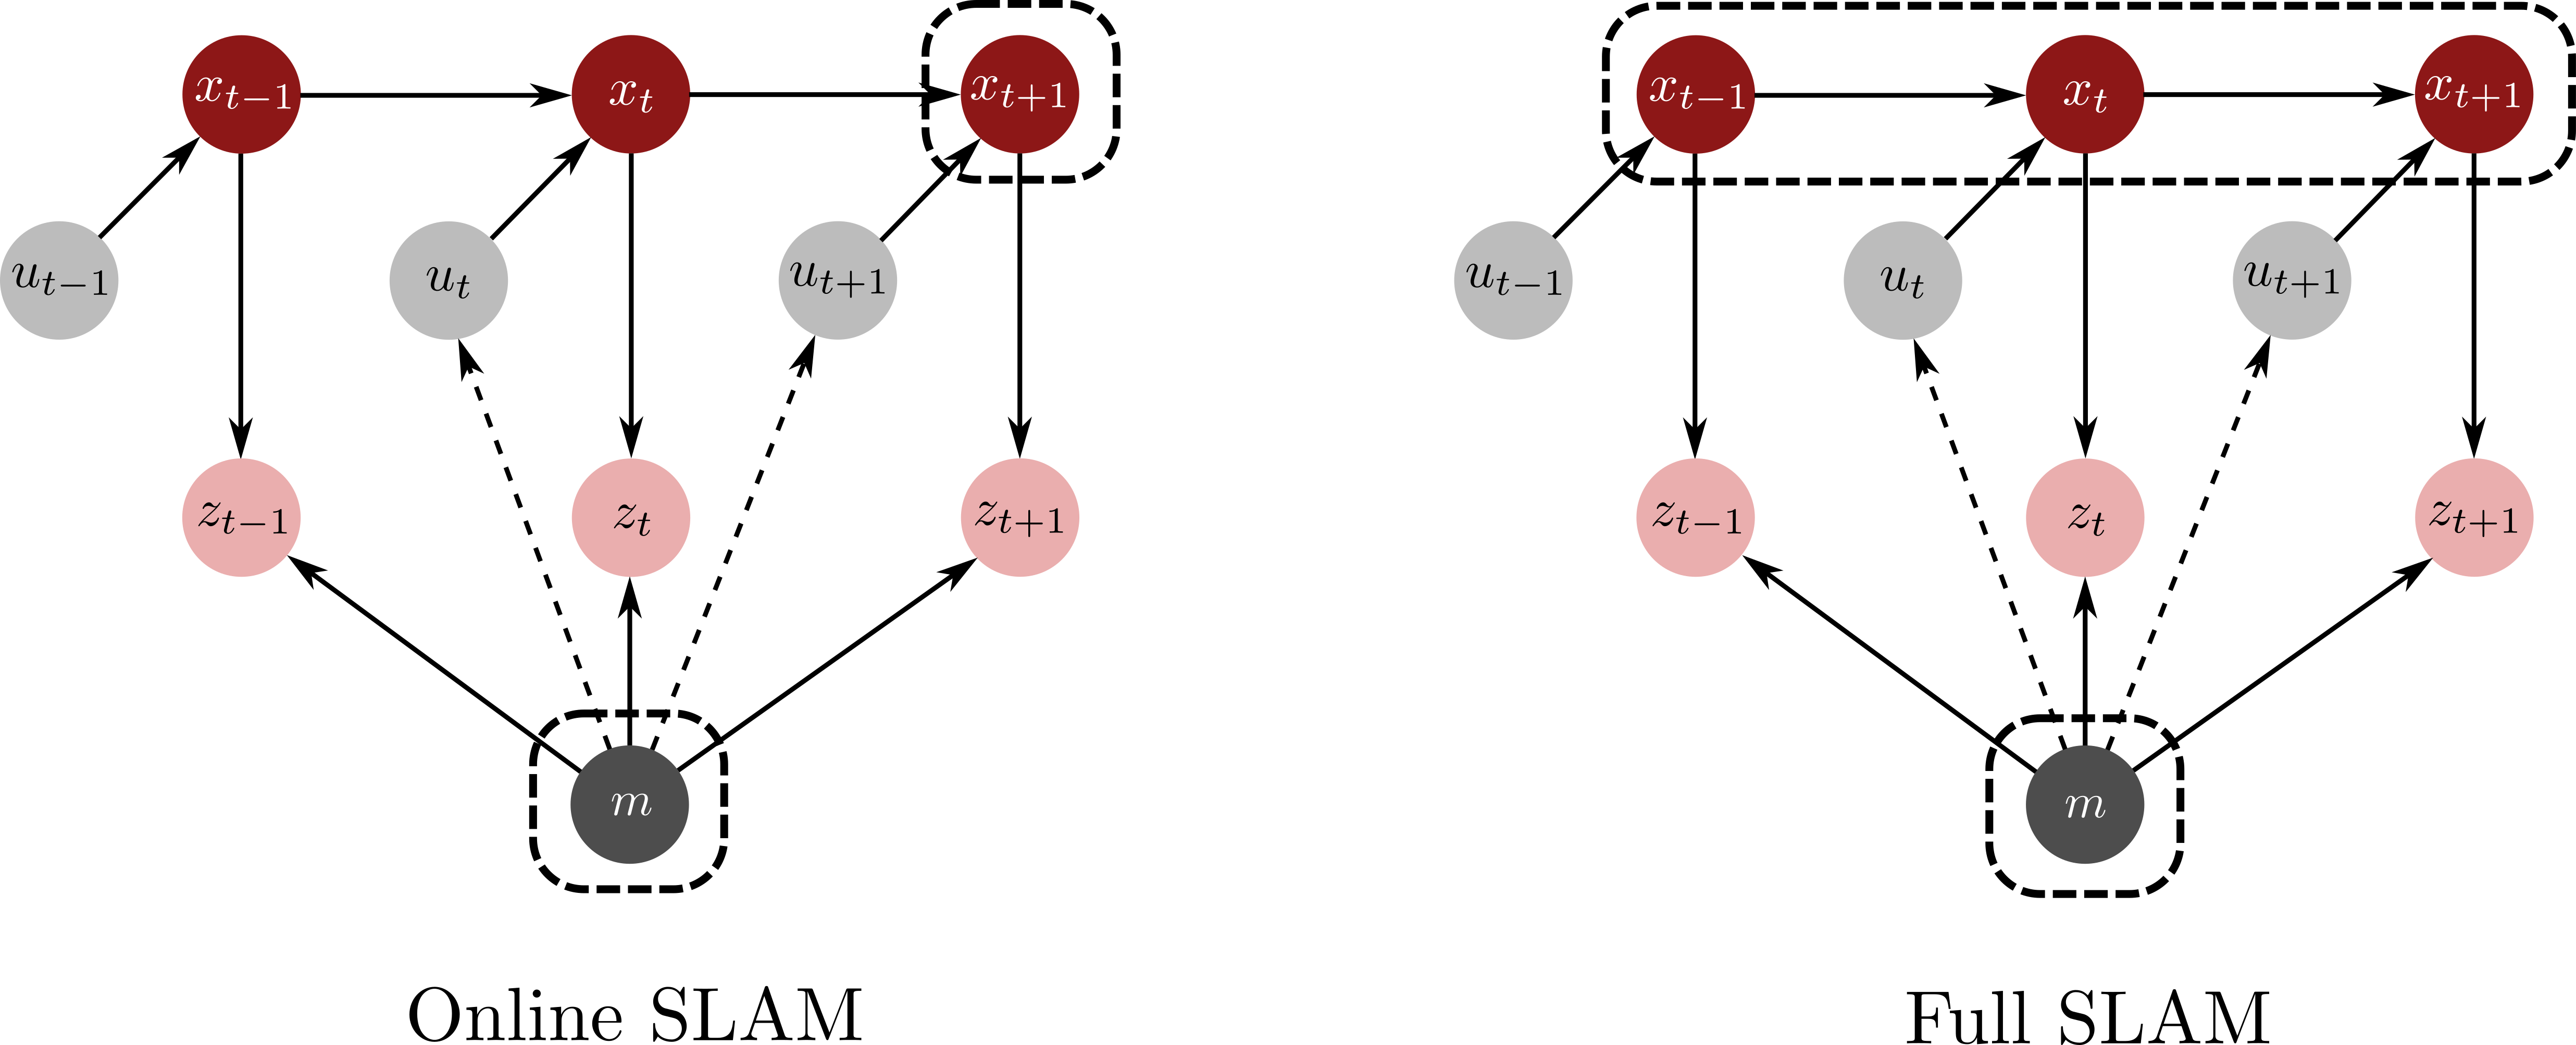
\includegraphics[width=.75\textwidth]{tex/figs/ch17_figs/online_full_slam.png}
    \caption{Difference between online and full SLAM, where online SLAM only estimates the current robot pose while full SLAM also estimates the robot's history.}
    \label{fig:online_full_slam}
\end{figure*}


\subsection{EKF SLAM Algorithm}
One of the earliest approaches to the online SLAM problem leverages the extended Kalman filter, and is essentially an extension of the EKF localization algorithm discussed in the previous chapter. Again, the key aspects to the approach are the exploitation of Gaussian distributions to model the robot's belief distribution $bel(\x_t)$, and state transition and measurement models.
It will also be assumed that the map is feature-based:
\begin{equation*}
\m = \{m_1,m_2,\dots ,m_N\},
\end{equation*}
where $m_i$ is the $i$-th landmark with coordinates $(m_{i,x}, m_{i,y})$. As in the EKF localization problem, the measurement correspondences can either be assumed to be known or unknown (more common in practice).

The main idea behind EKF SLAM is that the coordinates $(m_{i,x}, m_{i,y})$ of each landmark $m_i$ are added, along with the robot pose $\x_t$, to an augmented state vector:
\begin{equation} \label{eq:augmentedstate}
\y_t = \begin{bmatrix}
\x_t \\ \m_1 \\ \vdots \\ \m_N
\end{bmatrix},
\end{equation}
where $\m_i = [m_{i,x}, m_{i,y}]^\top $. With the new state vector $\y$ the online SLAM problem is to compute the posterior:
\begin{equation*}
bel(\y_t) = p(\y_t \mid \z_{1:t}, \bu_{1:t}).
\end{equation*}

EKF SLAM approaches have the advantage of being computationally efficient such that they can be run online, and are also well understood from a theoretical perspective. They can also provide good performance when the uncertainty is low. However, their main disadvantages are that they are restricted by the Gaussian assumption to unimodal estimates, and that performance can degrade in settings with high uncertainty or when the states are not well approximated by normal distributions.

\subsubsection{State Transition and Measurement Models}
Assuming that the landmarks $m_i \in \m$ are static, the state transition model for the augmented state vector $\y$ is assumed to be given by:
\begin{equation*}
    \y_t = g(\bu_t, \y_{t-1}) + \bm{\epsilon}_t, \quad \bm{\epsilon}_t \sim \mathcal{N}(\bm{0},\bm{R}_t),
\end{equation*}
where the nonlinear vector function $g$ is defined by:
\begin{equation*}
g(\bu_t, \y_{t-1}) = \begin{bmatrix}
\tilde{g}(\bu_t, \x_{t-1}) \\ \m_{1,t-1} \\ \vdots \\ \m_{N,t-1}
\end{bmatrix},
\end{equation*}
and $\tilde{g}$ is the original robot motion model (e.g. differential drive robot model). The noise covariance is also defined as:
\begin{equation*}
\bm{R}_t = \begin{bmatrix}
\tilde{\bm{R}}_t & 0 \\
0 & 0
\end{bmatrix},
\end{equation*}
where $\tilde{\bm{R}}_t$ is the noise covariance associated with the original robot motion model and the rest of the matrix are zeros.
The Jacobian of the augmented motion model is defined as $G_t \coloneqq \nabla_{\y} g(\bu_t, \bmu_{t-1})$ where $\bmu_{t-1}$ is the expected value of the belief distribution $bel(\y_{t-1})$ at the previous time.

The measurement model is defined in the same way as the previous chapter:
\begin{equation*}
\z^i_t = h(\y_t, j) + \bm{\delta}_t,
\end{equation*}
where $\bm{\delta}_t \sim \mathcal{N}(\bm{0}, \bm{Q}_t)$ is Gaussian zero-mean noise and $j$ is the index of the map feature $m_j \in \m$ that measurement $i$ is associated with. The Jacobian is also defined in the same way with $H^{j}_t = \nabla_{\y}h(\bar{\bmu}_t,j)$, where $\bar{\bmu}_t$ is the predicted mean (that results from the EKF prediction step) of the distribution $\overline{bel}(\y_t)$.

\subsubsection{EKF SLAM with Known Correspondences}
As was the case in EKF localization, it is important to specify whether the the correspondences $c_t^i$ between the $i$-th measurement $\z_t^i$ and the associated landmark in the map is known. In this section an EKF SLAM algorithm will be developed which assumes the correspondences $\bc_t = [c_t^1, \dots ]^\top $ are \textit{known}. 



\begin{algorithm}[ht]
 \KwData{$\bmu_{t-1}, \bSigma_{t-1}, \bu_{t}, \z_{t}, \bc_t$}
 \KwResult{$\bmu_t, \bSigma_t$}
 $\bar{\bmu}_t = g(\bu_t,\bmu_{t-1})$\\
 $\bar{\bSigma}_t = G_t\bSigma_{t-1} G_t^{T} + \bm{R}_t$\\
 \ForEach{$\z_t^i$}{
  $j = c_t^i$\\
  \If{landmark $j$ never seen before}{
    Initialize $\begin{bmatrix}\bar{\mu}_{j,x} \\ \bar{\mu}_{j,y} \end{bmatrix}$ as expected position based on $\z_t^i$
  }
  $S_t^i = H_t^j\bar{\bSigma}_{t}[H^j_t]^{T}+\bm{Q}_t$\\
  $K^i_t = \bar{\bSigma}_{t}[H^j_t]^{T}[S_t^i]^{-1}$\\
  $\bar{\bmu}_t = \bar{\bmu}_t + K^i_t(\z^i_t - h(\bar{\bmu}_{t}, j))$\\
  $\bar{\bSigma}_t = (I - K^i_t H^j_t)\bar{\bSigma}_t$\\
 }
 $\bmu_t = \bar{\bmu}_t$\\
 $\bSigma_t = \bar{\bSigma}_t$\\
 \Return $\bmu_t, \bSigma_t$
 \caption{Extended Kalman Filter Online SLAM Algorithm}
 \label{alg:ekfslam}
\end{algorithm}
Algorithm \ref{alg:ekfslam} presents the EKF SLAM algorithm with known correspondences. It is almost identical to the EKF localization algorithm from last chapter, except that the state vector is augmented with the landmark positions and the positions of these landmarks are initialized when they are first seen. For this algorithm a general initialization of the belief distribution $bel(\y_0)$ is with:
\begin{equation*}
\bmu_0 = \begin{bmatrix}
\x_0 \\ 0 \\ \vdots \\ 0
\end{bmatrix}, \quad \bSigma_0 = \begin{bmatrix}
\tilde{\bSigma}_0 & 0 & \cdots & 0 \\
    0 & \infty & \cdots & 0 \\
     \vdots & \vdots & \ddots & \vdots \\
    0 & 0 & \cdots & \infty \\
\end{bmatrix},
\end{equation*}
where:
\begin{equation*}
\x_0 = \begin{bmatrix}
0 \\ \vdots \\ 0
\end{bmatrix}, \quad \tilde{\bSigma}_0 = \begin{bmatrix}
0 & \cdots & 0 \\ \vdots & \ddots & \vdots \\ 0 & \cdots & 0
\end{bmatrix},
\end{equation*}
and $\x_0$ and $\tilde{\bSigma}$ are the initial robot state and associated covariance (which is set to zero).
Since the reference frame for the map can be defined arbitrarily, this initialization is used to say that the initial robot pose is known to be at the origin with certainty (and the map is built with respect to that origin). The covariance of the map positions is set to infinity to reflect that there is initially no knowledge of their position.




\subsection{EKF SLAM with Unknown Correspondences}
Performing EKF SLAM when the correspondences between measurements and landmarks are \textit{unknown} poses a more challenging problem. In the EKF localization case (when the map was known), a maximum likelihood method was used to determine correspondence. A similar approach is taken for EKF SLAM, which uses a maximum likelihood approach based on the \textit{estimated} landmark positions. The main difference is that now a mechanism for hypothesizing that a new landmark has been found is also required. The EKF SLAM with unknown correspondences algorithm is given in Algorithm \ref{alg:ekfslamunknowncorr}.
\begin{algorithm}[ht]
 \KwData{$\bmu_{t-1}, \bSigma_{t-1}, \bu_{t},\z_{t}, N_{t-1}$}
 \KwResult{$\bmu_t, \bSigma_t$}
 $N_t = N_{t-1}$\\
 $\bar{\bmu}_t = g(\bu_t,\bmu_{t-1})$\\
 $\bar{\bSigma}_t = G_t\bSigma_{t-1} G_t^{T} + \bm{R}_t$\\
 \ForEach{$\z_t^i$}{
  Hypothesize position $\begin{bmatrix}\bar{\mu}_{N_t + 1,x} \\ \bar{\mu}_{N_t + 1,y} \end{bmatrix}$ from $\z_t^i$ \\
    \ForEach{$k=1$ \KwTo $N_t+1$}{
      $\hat{\z}_t^k = h(\bar{\bmu}_{t}, k)$\\
      $S_t^k = H_t^k\bar{\bSigma}_{t}[H^k_t]^{T}+\bm{Q}_t$\\
      $d_t^{ik} = (\z_t^i-\hat{\z}^{k}_t)^\top  [S_t^{k}]^{-1} (\z_t^i-\hat{\z}^{k}_t)$\\
     }
  $d_t^{i(N_t+1)} = \alpha$\\
  $j = \arg\min_k \:\: d_t^{ik}$\\
  $N_t = \max \{N_t, j\}$\\
  $K^i_t = \bar{\bSigma}_{t}[H^j_t]^{T}[S_t^j]^{-1}$\\
  $\bar{\bmu}_t = \bar{\bmu}_t + K^i_t(\z^i_t - \hat{\z}_t^j)$\\
  $\bar{\bSigma}_t = (I - K^i_t H^j_t)\bar{\bSigma}_t$\\
 }
 $\bmu_t = \bar{\bmu}_t$\\
 $\bSigma_t = \bar{\bSigma}_t$\\
 \Return $\bmu_t, \bSigma_t$
 \caption{EKF Online SLAM Algorithm, Unknown Correspondences}
 \label{alg:ekfslamunknowncorr}
\end{algorithm}

As can be seen there are a couple differences between Algorithm \ref{alg:ekfslam} and Algorithm \ref{alg:ekfslamunknowncorr}. First, the measurements $\z_k^i$ are used to \textit{hypothesize} the position of a new landmark. The Mahalanobis distance $d_t^{ik}$ is then computed for all currently tracked landmarks, and the hypothesized landmark is added if the distance exceeds a threshold $\alpha$ (i.e. $d_t^{ik} > \alpha$ for all $k = 1,\dots,N_t$).


While this EKF-based algorithm can be used to solve the online SLAM problem without correspondences, it is not necessarily the most robust approach. In particular, extraneous measurements can result in the creation of fake landmarks, which will then propagate forward to future steps and cannot be corrected!
There are several techniques to mitigate these issues, such as using outlier rejection schemes or strategies to enhance the distinctiveness of landmarks (which may require prior knowledge or assumptions).
Another important disadvantage of EKF SLAM is that its computational complexity is quadratic with the number of landmarks $N$, but generally a large number of landmarks is required for good localization accuracy!


\begin{example}[Differential Drive Robot with Range and Bearing Measurements] \label{ex:rangeandbearingEKFSLAM}
\theoremstyle{definition}
Consider a differential drive robot with state $\x = [x, y, \theta]^\top $, and suppose a sensor is available on the robot which measures the range $r$ and bearing $\phi$ of landmarks $m_j \in \m$ relative to the robot’s local coordinate frame. Additionally, multiple measurements corresponding to different features can be collected at each time step:
\begin{equation*}
\z_t = \{[r_t^1,\phi_t^1]^\top , [r_t^2,\phi_t^2]^\top , \dots\},
\end{equation*}
where each measurement $\z_t^i$ contains the range $r_t^i$ and bearing $\phi_t^i$. 

For the SLAM problem, the augmented state $\y_t$ is defined as:
\begin{equation*}
\y_t =
    \begin{bmatrix}
    \x_t \\
    \m_1 \\ \vdots \\ \m_N
    \end{bmatrix}
    = \begin{bmatrix}
    x & y & \theta & m_{1,x} &m_{1,y} & \dots & m_{N,x} &m_{N,y}
    \end{bmatrix}^\top .
\end{equation*}

Assuming the correspondences are known, the measurement model for the range and bearing is:
\begin{equation}
h(\y_t, j)  = \begin{bmatrix}
\sqrt{(m_{j,x} - x)^{2} + (m_{j,y}- y)^{2}} \\
\text{atan2}(m_{j,y}- y, m_{j,x} - x) - \theta
\end{bmatrix}.
\end{equation}
The measurement Jacobian $H^j_t$ corresponding to a measurement from landmark $j$ is then given by:
\begin{equation}
H^j_t = \begin{bmatrix}
-\frac{\bar{\mu}_{j,x} - \bar{\mu}_{t,x}}{\sqrt{q_{t,j}}} & -\frac{\bar{\mu}_{j,y} - \bar{\mu}_{t,y}}{\sqrt{q_{t,j}}} & 0 & 0 & \dots & 0 & \frac{\bar{\mu}_{j,x} - \bar{\mu}_{t,x}}{\sqrt{q_{t,j}}} & \frac{\bar{\mu}_{j,y} - \bar{\mu}_{t,y}}{\sqrt{q_{t,j}}} & 0 & \dots \\
\frac{\bar{\mu}_{j,y} - \bar{\mu}_{t,y}}{q_{t,j}} & -\frac{\bar{\mu}_{j,x} - \bar{\mu}_{t,x}}{q_{t,j}} & -1 & 0 & \dots & 0 & -\frac{\bar{\mu}_{j,y} - \bar{\mu}_{t,y}}{q_{t,j}} & \frac{\bar{\mu}_{j,x} - \bar{\mu}_{t,x}}{q_{t,j}} & 0 & \dots 
\end{bmatrix},
\end{equation}
where:
\begin{equation*}
    q_{t,j} := (\bar{\mu}_{j,x} - \bar{\mu}_{t,x})^{2} + (\bar{\mu}_{j,y} - \bar{\mu}_{t,y})^{2},
\end{equation*}
and $\bar{\mu}_{j,x}$ and $\bar{\mu}_{j,y}$ are the estimate of the $x$ and $y$ coordinates of landmark $m_j$ from $\bar{\bmu}_t$.

With both a range and bearing measurement, the \textit{expected} position of landmark $m_j$ is given by:
\begin{equation*}
    \begin{bmatrix}
    \bar{\mu}_{j,x} \\
    \bar{\mu}_{j,y}
    \end{bmatrix}
    = \begin{bmatrix}
    \bar{\mu}_{t,x}\\
    \bar{\mu}_{j,y}
    \end{bmatrix}
    +
    \begin{bmatrix}
    r^{i}_{t}\text{cos}(\phi^{i}_{t} + \bar{\mu}_{t,\theta}) \\
    r^{i}_{t}\text{sin}(\phi^{i}_{t} + \bar{\mu}_{t,\theta})
    \end{bmatrix}.
\end{equation*}
This can be used in the known-correspondence EKF SLAM algorithm (Algorithm \ref{alg:ekfslam}) to initialize the landmark position and can be used in the unknown-correspondence case (Algorithm \ref{alg:ekfslamunknowncorr}) to hypothesize the position of new landmarks.
\end{example}


\subsection{Particle SLAM Algorithm}
Another approach to the robot SLAM problem is to leverage the non-parametric particle filter. In fact, particle SLAM can be used to solve the \textit{full} SLAM problem, unlike EKF SLAM which only solves the online SLAM problem. Specifically, the full SLAM problem is to estimate the posterior distribution $p(\x_{1:t}, \m \mid \z_{1:t}, \bu_{1:t})$, which includes the full robot path $\x_{1:t}$ up to time $t$ and the map $\m$. Similar to the EKF SLAM case, the robot state $\x_{1:t}$ and map feature positions $\m$ are combined into an augmented state vector $\y_{1:t}$ as in \eqref{eq:augmentedstate}.

A na\"ive implementation of the particle filter in the context of full SLAM would be computationally intractable, since the number of particles required to belief distribution would be extremely large. However, the key insight that makes this approach tractable is that the posterior over the map elements is \textit{conditionally independent} given the true path of the robot. Therefore the mapping component to the problem can be split up into separate problems, corresponding to each feature in the map! Splitting the problem in this way makes the overall problem much easier to solve.

Overall, particle filter SLAM approaches can be used with \textit{any} noise distribution and can express multimodal beliefs since they are non-parametric. Additionally, in practice they can be relatively easy to implement and can also be more robust to data association errors. Their main disadvantages are that they typically do not scale well to large scale problems (too many particles are needed), and that without enough particles convergence may not occur.

\subsubsection{Factoring the Posterior}
The key insight of particle SLAM that makes it a computationally tractable algorithm is that the posterior $p(\y_{1:t} \mid \z_{1:t}, \bu_{1:t}, c_{1:t})$ can be factored as:
\begin{equation} \label{eq:factored}
p(\y_{1:t} \mid \z_{1:t}, \bu_{1:t}, c_{1:t}) = p(\x_{1:t} \mid \z_{1:t}, \bu_{1:t}, c_{1:t}) \prod_{n=1}^N p(\m_n \mid \x_{1:t}, \z_{1:t},  c_{1:t}),    
\end{equation}
where $\m_n$ is the $n$-th feature in the map $\m$, the term $p(\x_{1:t} \mid \z_{1:t}, \bu_{1:t}, c_{1:t})$ is referred to as the \textit{path posterior}, and the terms $p(\m_n \mid \x_{1:t}, \z_{1:t},  c_{1:t})$ are referred to as the \textit{feature posteriors}. 

This factorization can be derived by first using Bayes' rule
\begin{equation*}
p(\y_{1:t} \mid \z_{1:t}, \bu_{1:t}, c_{1:t}) = p(\x_{1:t} \mid \z_{1:t}, \bu_{1:t}, c_{1:t}) p(\m \mid \x_{1:t}, \z_{1:t}, \bu_{1:t},  c_{1:t}),    
\end{equation*}
and then noting that since the feature posterior is conditioned on $\x_{1:t}$, the dependence on $\bu_{1:t}$ is redundant:\begin{equation*}
p(\y_{1:t} \mid \z_{1:t}, \bu_{1:t}, c_{1:t}) = p(\x_{1:t} \mid \z_{1:t}, \bu_{1:t}, c_{1:t}) p(\m \mid \x_{1:t}, \z_{1:t},  c_{1:t}).
\end{equation*}

Now the feature posterior $p(\m \mid \x_{1:t}, \z_{1:t},  c_{1:t})$ can be explored in more detail. In particular two cases can be considered for each landmark $\m_n$: the case when the measurement at time $t$ is not associated with $n$ and the case when it is:
\begin{equation*}
p(\m_n \mid \x_{1:t}, \z_{1:t}, c_{1:t}) = \begin{cases}
p(\m_n \mid \x_{1:t-1}, \z_{1:t-1},  c_{1:t-1}), \quad &c_t \neq n, \\
\frac{p(\z_t \mid \m_n, \x_{t}, c_{t})p(\m_n \mid \x_{1:t-1}, \z_{1:t-1}, c_{1:t-1})}{p(\z_t \mid \x_{1:t}, \z_{1:t-1}, c_{1:t})}, \quad &c_t = n,
\end{cases}
\end{equation*}
where in the second case Bayes' rule was applied. It is now possible to show the result \eqref{eq:factored} by induction. First, suppose that:
\begin{equation*}
p(\m \mid \x_{1:t-1}, \z_{1:t-1},  c_{1:t-1}) = \prod_{n=1}^N p(\m_n \mid \x_{1:t-1}, \z_{1:t-1},  c_{1:t-1}).
\end{equation*}
Then, using Bayes' rule at time $t$:
\begin{equation*}
\begin{split}
p(\m \mid \x_{1:t}, \z_{1:t}, c_{1:t}) &= \frac{p(\z_t \mid \m, \x_{t}, c_{t})p(\m \mid \x_{1:t-1}, \z_{1:t-1}, c_{1:t-1})}{p(\z_t \mid \x_{1:t}, \z_{1:t-1}, c_{1:t})}, \\
&= \frac{p(\z_t \mid \m, \x_{t}, c_{t})}{p(\z_t \mid \x_{1:t}, \z_{1:t-1}, c_{1:t})} \prod_{n=1}^N p(\m_n \mid \x_{1:t-1}, \z_{1:t-1},  c_{1:t-1}). \\
\end{split}
\end{equation*}
Next, applying the analysis above for the cases where $c_t \neq n$ and $c_t = n$:
\begin{equation*}
\begin{split}
p(\m \mid \x_{1:t}, \z_{1:t}, c_{1:t}) &= p(\m_{c_t} \mid \x_{1:t}, \z_{1:t},  c_{1:t}) \prod_{n\neq c_t} p(\m_n \mid \x_{1:t}, \z_{1:t},  c_{1:t}), \\
&= \prod_{n=1}^N p(\m_n \mid \x_{1:t}, \z_{1:t},  c_{1:t}). \\
\end{split}
\end{equation*}

\subsubsection{Fast SLAM with Known Correspondences}
The particle SLAM algorithm referred to as Fast SLAM uses the factorization of the posterior $p(\y_{1:t} \mid \z_{1:t}, \bu_{1:t}, c_{1:t})$ in \eqref{eq:factored} to decompose the full SLAM problem into more manageable sub-problems. Specifically, the path posterior $p(\x_{1:t} \mid \z_{1:t}, \bu_{1:t}, c_{1:t})$ is estimated using a particle filter and the feature posteriors $p(\m_n \mid \x_{1:t}, \z_{1:t},  c_{1:t})$ are estimated by EKFs conditioned on the robot path $\x_{1:t}$ (i.e. there is a separate EKF for each feature $\m_n$).

Accordingly, the set of particles is given as:
\begin{equation*}
\mathcal{Y}_t \coloneqq \{Y_t^{[1]}, Y_t^{[2]},..., Y_t^{[M]}\},
\end{equation*}
where the $k$-th particle is defined by:
\begin{equation*}
Y_t^{[k]} = \{\x_t^{[k]}, \bmu_{1,t}^{[k]}, \bSigma_{1,t}^{[k]}, \dots, \bmu_{N,t}^{[k]}, \bSigma_{N,t}^{[k]} \},
\end{equation*}
where $\x_t^{[k]}$ is a hypothesis of the robot state at time $t$, $(\bmu_{n,t}^{[k]}, \bSigma_{n,t}^{[k]})$ are the mean and covariance of the EKF associated with landmark $\m_n$, and where it is assumed that there are $N$ total landmarks in the map $\m$. As can be seen, with a total of $M$ particles there are a total of $NM$ EKFs!
To summarize, the Fast SLAM algorithm is a particle based algorithm where each particle keeps track of a hypothesis of the robot state as well as the location (and uncertainty) of each landmark in the map! The algorithm is defined in Algorithm \ref{alg:fastslam}.
\begin{algorithm}[ht]
 \KwData{$\mathcal{Y}_{t-1}, \bu_{t}, \z_{t}, c_t$}
 \KwResult{$\mathcal{Y}_{t}$}
 \For{$k=1$ \KwTo $M$}{
  Sample $\x_{t}^{[k]} \sim p(\x_t\mid \bu_t, \x_{t-1}^{[k]})$\\
  $j = c_t$\\
  \eIf{landmark $j$ never seen before}{
    Initialize feature: $(\bmu^{[k]}_{j,t-1}, \bSigma^{[k]}_{j,t-1})$
  }
  {
  $\hat{\z}^{[k]} = h(\bmu^{[k]}_{j,t-1}, \x_{t}^{[k]})$\\
  $S = H^j\bSigma^{[k]}_{j,t-1}[H^j]^{T}+\bm{Q}_t$\\
  $K = \bSigma^{[k]}_{j,t-1}[H^j]^{T}[S]^{-1}$\\
  $\bmu^{[k]}_{j,t} = \bmu^{[k]}_{j,t-1} + K(\z_t - \hat{\z}^{[k]})$\\
  $\bSigma^{[k]}_{j,t} = (I - K H^j)\bSigma^{[k]}_{j,t-1}$\\
  $w^{[k]} = \text{det}(2\pi S)^{-1/2}\text{exp}\big(-\frac{1}{2}(\z_t - \hat{\z}^{[k]})\bm{Q}^{-1}(\z_t - \hat{\z}^{[k]})\big)$\\
  }
  \For{$n \in \{1,\dots,N\}$, $n \neq c_t$}{
  $\bmu^{[k]}_{n,t} = \bmu^{[k]}_{n,t-1}$\\
  $\bSigma^{[k]}_{n,t} = \bSigma^{[k]}_{n,t-1}$\\
 }
 }
 $\mathcal{Y}_t = \emptyset$\\
 \For{$m=1$ \KwTo $M$}{
  Draw $k$ with probability $\propto w_t^{[k]}$\\
  $\mathcal{Y}_t = \mathcal{Y}_t \cup (\bar{\x}_{t}^{[k]}, \bmu^{[k]}_{1,t}, \bSigma^{[k]}_{1,t}, \dots, \bmu^{[k]}_{N,t}, \bSigma^{[k]}_{N,t})$\\
 }
 \Return $\mathcal{Y}_t$
 \caption{Fast SLAM Algorithm}
 \label{alg:fastslam}
\end{algorithm}

Note the blending of the classical particle filter algorithm with the EKF localization algorithm. In particular, the particle filter steps can be seen with the sampling of the new pose $\x_t$ from the state transition model and the use of the weights $w$ for resampling a new set of particles (i.e. the measurement correction step). The EKF portions of the algorithm correspond to how the features are tracked, and in particular how the mean and covariance of the Gaussian corresponding to each landmark are updated based on new measurements.

\subsection{Exercises}
\subsubsection{EKF SLAM}
Complete \textit{Problem 2: EKF SLAM} located in the online repository:

\vspace{\baselineskip}

\url{https://github.com/PrinciplesofRobotAutonomy/AA274A_HW4},

\vspace{\baselineskip}

where you will implement an EKF SLAM algorithm. Note that the EKF localization exercise from the chapter on parametric filters should be completed first.

